\documentclass[]{article}
\usepackage{lmodern}
\usepackage{amssymb,amsmath}
\usepackage{ifxetex,ifluatex}
\usepackage{fixltx2e} % provides \textsubscript
\ifnum 0\ifxetex 1\fi\ifluatex 1\fi=0 % if pdftex
  \usepackage[T1]{fontenc}
  \usepackage[utf8]{inputenc}
\else % if luatex or xelatex
  \ifxetex
    \usepackage{mathspec}
  \else
    \usepackage{fontspec}
  \fi
  \defaultfontfeatures{Ligatures=TeX,Scale=MatchLowercase}
\fi
% use upquote if available, for straight quotes in verbatim environments
\IfFileExists{upquote.sty}{\usepackage{upquote}}{}
% use microtype if available
\IfFileExists{microtype.sty}{%
\usepackage{microtype}
\UseMicrotypeSet[protrusion]{basicmath} % disable protrusion for tt fonts
}{}
\usepackage[margin=1in]{geometry}
\usepackage{hyperref}
\hypersetup{unicode=true,
            pdftitle={Detecting marine heatwaves},
            pdfauthor={Robert W. Schlegel, Eric C. J. Oliver, Alistair J. Hobday, Albertus J. Smit},
            pdfborder={0 0 0},
            breaklinks=true}
\urlstyle{same}  % don't use monospace font for urls
\usepackage{graphicx,grffile}
\makeatletter
\def\maxwidth{\ifdim\Gin@nat@width>\linewidth\linewidth\else\Gin@nat@width\fi}
\def\maxheight{\ifdim\Gin@nat@height>\textheight\textheight\else\Gin@nat@height\fi}
\makeatother
% Scale images if necessary, so that they will not overflow the page
% margins by default, and it is still possible to overwrite the defaults
% using explicit options in \includegraphics[width, height, ...]{}
\setkeys{Gin}{width=\maxwidth,height=\maxheight,keepaspectratio}
\IfFileExists{parskip.sty}{%
\usepackage{parskip}
}{% else
\setlength{\parindent}{0pt}
\setlength{\parskip}{6pt plus 2pt minus 1pt}
}
\setlength{\emergencystretch}{3em}  % prevent overfull lines
\providecommand{\tightlist}{%
  \setlength{\itemsep}{0pt}\setlength{\parskip}{0pt}}
\setcounter{secnumdepth}{0}
% Redefines (sub)paragraphs to behave more like sections
\ifx\paragraph\undefined\else
\let\oldparagraph\paragraph
\renewcommand{\paragraph}[1]{\oldparagraph{#1}\mbox{}}
\fi
\ifx\subparagraph\undefined\else
\let\oldsubparagraph\subparagraph
\renewcommand{\subparagraph}[1]{\oldsubparagraph{#1}\mbox{}}
\fi

%%% Use protect on footnotes to avoid problems with footnotes in titles
\let\rmarkdownfootnote\footnote%
\def\footnote{\protect\rmarkdownfootnote}

%%% Change title format to be more compact
\usepackage{titling}

% Create subtitle command for use in maketitle
\newcommand{\subtitle}[1]{
  \posttitle{
    \begin{center}\large#1\end{center}
    }
}

\setlength{\droptitle}{-2em}

  \title{Detecting marine heatwaves}
    \pretitle{\vspace{\droptitle}\centering\huge}
  \posttitle{\par}
    \author{Robert W. Schlegel, Eric C. J. Oliver, Alistair J. Hobday, Albertus J.
Smit}
    \preauthor{\centering\large\emph}
  \postauthor{\par}
      \predate{\centering\large\emph}
  \postdate{\par}
    \date{25 May 2018}


\begin{document}
\maketitle

\section{Abstract}\label{abstract}

It is now known that marine heatwaves (MHWs) have been increasing in
duration and intensity globally for decades, implying that the
destruction that follows in their wake is increasing, too. There are
many documented instances of such destruction however, there are many
ocean, sea, and coastal regions where our ability to accurately detect
events is uncertain because they have not been sampled continuously for
30 or more years, as is the standard recommendation. It was therefore
necessary to quantify the effect that short time series duration or
missing data may have on the accurate detection of MHWs where optimal
data are not available. It was found that time series as short as 10
years had little effect on the duration or intensities of events
detected, but the accurate creation of the 90th percentile thresholds
was impaired when fewer than \textasciitilde{}25 years of data were
used. It was also found that the categories of MHWs detected in time
series missing 15 -- 25\% of their data did not differ significantly
from those detected in complete time series. It was also found that
linear decadal trends as low as 0.10°C/dec could lead to inaccurate
creation of seasonal climatologies, but that this did not impact
accurate event detection. The percentage of missing data in a time
series was determined to have the most dramatic effect on the accurate
detection of events. The best practices for how to improve the accuracy
of MHW detection with sub-optimal time series has been itemised and is
discussed in detail here using specific case studies of three notable
MHWs from the literature as workable examples.

\section{Introduction}\label{introduction}

The idea of hot seawater being problematic is not a novel concept. We
have known for decades, perhaps millennia, that seemingly transient
occurrences in the ocean could leave ecosystems barrens with no notice
of the event until the waters had already cooled. It was perhaps due to
our lack of ability to track and record ocean temperatures globally that
people did not begin to quantify the effects of anomalously warm
seawater temperatures until the mid 90s (cite). It was not until the
00's that much work began to be done on the direct consequences of this
hot water (e.g. Garrabou et al. 2009). Later still was the development
of a globally utilised definition for these events that enjoyed
wide-spread use. The now commonly used Alistair J. Hobday et al. (2016)
definition for anomalously warm seawater temperature events, better
known as marine heatwaves (MHWs) has allowed researchers around the
world to directly compare events in very different environments for the
present as well as the past. A follow up to this definition has now also
introduced a category naming convention (Alistair J Hobday et al. 2018)
that makes the application of this definition even more useful for
transdisciplinary work.

\begin{itemize}
\tightlist
\item
  \emph{I'm willing to write a more conventional paragraph below if
  everyone would prefer.}
\end{itemize}

It is perhaps belaboring the point to explain the danger that MHWs pose
to the world, so below is a brief bulleted list outlining some of the
more well studied MHWs and the impacts they have had:

\begin{itemize}
\tightlist
\item
  Mediterranean 2008: (Garrabou et al., 2009; Olita et al., 2007)
\item
  South West coast of Australia 2010/11: (Feng et al., 2013; Pearce and
  Feng, 2013; Wernberg et al., 2013)
\item
  Northwest Atlantic 2012: (Chen et al., 2014, 2015; Mills et al., 2012)
\item
  ``The Blob'' Northeast Pacific Ocean 2013-16: (Bond et al., 2015)
\item
  Tasman Sea in 2015/16: (cite)
\item
  waters around tropical Australia in 2015/16: (cite)
\end{itemize}

\section{Marine heatwaves thus far}\label{marine-heatwaves-thus-far}

The Alistair J. Hobday et al. (2016) definition for MHWs is best summed
up as ``A prolonged discrete anomalously warm water event that can be
described by its duration, intensity, rate of evolution, and spatial
extent.''. Accompanying this definition is an algorithm that produces a
suite of metrics that researchers may use to define the events and to
effectively compare them against known ecological/financial impacts
using an ever-growing list of statistical tools. A full explanation for
these metrics may be found in Table 2 of Alistair J. Hobday et al.
(2016).

A common definition for MHWs was necessary because as they begin to
increase in duration and intensity around the world (Oliver et al.
2018), the research of different groups will be able to directly benefit
from cross-comparison of results. For example, a mean intensity of 2°C
for at least XXX days may be damaging to a range of coral species
(cite). Using this research from the Great Barrier Reef, a team in the
Caribbean may now have a better idea of what to look out for with
regards to their own research.

It is perhaps due to the ease and interoperability of this methodology
that it has seen rapidly increasing use across marine sciences (cite?).
This has introduced a new series of meta-issues in that different groups
often depart from the default use of the algorithm for MHW detection in
varying degrees (e.g.~cite Spanish paper), or simply use entirely
different methodologies (e.g. Frölicher, Fischer, and Gruber 2018) while
referring to the Alistair J. Hobday et al. (2016) definition. This has
given rise to concerns over best practices. What should a group do if
faced with a particular challenge, such as wanting to use an \emph{in
situ} collected time series of bottom temperatures that is only 15 years
old? Or perhaps using a time series that is collected by hand during
only weekdays, and not weekends? These are real issues that need
answers.

Before we outline the issues we intend to address below, it must be
stressed that this list is neither exhaustive, nor is it meant to be
perceived as authoritative. However one chooses to quantify MHWs will be
of benefit to the scientific community. The issues that we work out in
this paper are designed to ensure that the use of the Alistair J. Hobday
et al. (2016) and Alistair J Hobday et al. (2018) methodology will
remain comparable even if performed with data that do not meet the
minimum requirements that were first proscribe. The definition of a MHW
is naturally evolving as our tools for detection advance and so the
definition itself is not set in stone any more than is necessary to
ensure backwards compatibility with previously published research.

\section{Outstanding issues}\label{outstanding-issues}

There are a number of issues that were not within the scope of either
Alistair J. Hobday et al. (2016) or Alistair J Hobday et al. (2018) to
address that we seek to investigate here. This breaks down into two main
topics. The first topic is what can be done when a researcher wants to
use a time series, but it does not meet the proscribed minimum
requirements of: 1) 30 years and 2) no missing days. There are a number
of methods within the already existing arsenal of tools that can address
these concerns and we will lay them out here. The second broad topic is
to determine how much of an effect long-term trends have on the accurate
detection of events. Oliver et al. (2018) has shown how dominant the
climate change signal can be in the detection of events and we seek to
break that down here, quantifying its effects in an informative manner.

A final issue for consideration before beginning to investigate the
outstanding issues outlined above was to ensure that the results
generated for MHW detection from any programming language would be the
same. The MHW algorithm is currently available in
\href{https://github.com/ecjoliver/marineHeatWaves}{python}(cite),
\href{https://cran.r-project.org/web/packages/heatwaveR/index.html}{R}(cite),
and \href{https://github.com/ZijieZhaoMMHW/m_mhw1.0}{MATLAB}(cite). For
this analysis we compared the R and python
\href{https://robwschlegel.github.io/MHWdetection/articles/r_vs_python.html}{default}
outputs, how changing the
\href{https://robwschlegel.github.io/MHWdetection/articles/r_vs_python_arguments.html}{arguments}
affected the default outputs, as well as a comparison of the other
\href{https://robwschlegel.github.io/MHWdetection/articles/r_vs_python_additional.html}{functionality}
provided between the two languages. It was found that while some style
differences exist between the added functionality of the languages, the
core climatology outputs are identical to within \textless{} 0.001 °C
per day-of-year (doy). An independent analysis of the Python and MATLAB
results also confirmed that they were functionally identical (pers. com.
Zijie Zhao; MATLAB distribution author).

Before outlining the methodology used in this paper, we have summarised
some of the more commonly used data products for the detection of MHWs
and what potential issues they may have. This information may then be
used by the reader to more readily see which fixes may be most useful
for them.

It must be mentioned that while this paper seeks to investigate the best
practices for the application of the Alistair J. Hobday et al. (2016)
and Alistair J Hobday et al. (2018) definition for MHWs, this may also
be done independently and there should be no obstacle to researchers
obtaining comparable results using their own implementation of these
ideas.

\section{Useful data for MHW
detection}\label{useful-data-for-mhw-detection}

\begin{itemize}
\tightlist
\item
  \emph{I'm thinking that the data summary section should be removed or
  severely shorteneds}

  \begin{itemize}
  \tightlist
  \item
    \emph{Perhaps just talk about the three broad categories and what
    their advantages and disadvantages are}
  \end{itemize}
\end{itemize}

Outlined here in a series of three tables are a non-exhaustive list of
the products currently available for work with MHW detection. The
advantages, disadvantages, and any known issues are listed with the
products in addition to a brief summary of their meta-data and where
they may be downloaded. The products are broken up into three broad
categories: remotely sensed data, reanalysis data, and \emph{ins situ}
data.

\begin{itemize}
\tightlist
\item
  \emph{In each table we can list the most common products that may be
  used at this time advantages would obviously be things like global
  vs.~point location (satellite), inclusion of subsurface data
  (reanalysis), resolution of coastal processes (in situ). Disadvantages
  around interpolation, resolution, missing data, time series length,
  etc\ldots{}}
\item
  \emph{Maybe insert a table here that lists all of the data sets that
  might be potentially useful, if we can overcome some of their
  limitation; in the table, also mention each product's limitations
  (e.g.~too short, too many NAs, etc.)}
\item
  \emph{Many gridded daily SST products are available that may make them
  more useful closer to the coast (but see Smit et al., 2013; etc.) due
  to their finer grid size (1-4km refs.), but the data do not yet cover
  a full 30 year period}
\item
  \emph{The finer resolution AVHRR data (4km) also run from 1981, but it
  is dodgy here off the coast of SA, and probably also elsewhere}
\item
  \emph{The various flavours of MODIS data are okay, but the time series
  only runs from the early 1990s. They are better near the coast, but
  not perfect.}
\item
  \emph{More recently people have started using the MUR and G1SST data,
  which at a resolution of 1 km resolve details in the coastal areas and
  look promising, but have not really been widely validated}
\item
  \emph{Many of these newer data sets are close to around 10 years
  long.}
\end{itemize}

Table 1: \textbar{}Remotely sensed data \textbar{}Description
\textbar{}Spatial res. \textbar{}Temporal res. \textbar{}Start date
\textbar{}End date \textbar{}Update \textbar{}Advantages
\textbar{}Disadvantages \textbar{}Solutions \textbar{}Download
\textbar{}
\textbar{}------------------\textbar{}------------------------------------------------\textbar{}----------\textbar{}--------\textbar{}--------\textbar{}-------\textbar{}------\textbar{}------\textbar{}------\textbar{}-------\textbar{}-------\textbar{}
\textbar{}NOAA OISST \textbar{}The NOAA optimally interpolated SST
(OISST) data (Reynolds et al. 2007) are currently the most commonly used
for the detection of MHWs. This product is corrected with the use
\emph{in situ} collected data, which are also used to fill gaps in the
record. \textbar{}0.25° (\textasciitilde{}25 km) global grid
\textbar{}Daily \textbar{}1981-09-01 \textbar{}Near real-time
\textbar{}Gapless global 30+ year time series \textbar{}Course
resolution and interpolation of data over gaps. Not suitable for use
within one pixel of a coastline. \textbar{}\ldots{}
\textbar{}www.ncdc.noaa.gov/oisst/data-access \textbar{} \textbar{}MODIS
AQUA \textbar{} \textbar{}MODIS TERRA \textbar{} \textbar{}AVHRR
Pathfinder v5.2 \textbar{} \textbar{}G1SST \textbar{} \textbar{}MUR
\textbar{}

Table 2: \textbar{}Reanalysis data \textbar{}Description
\textbar{}Spatial res. \textbar{}Temporal res. \textbar{}Start date
\textbar{}End date \textbar{}Update \textbar{}Advantages
\textbar{}Disadvantages \textbar{}Solutions \textbar{}Download
\textbar{}
\textbar{}------------------\textbar{}------------------------------------------------\textbar{}----------\textbar{}--------\textbar{}--------\textbar{}-------\textbar{}------\textbar{}------\textbar{}------\textbar{}-------\textbar{}-------\textbar{}
\textbar{}BRAN \textbar{}

\begin{itemize}
\tightlist
\item
  \emph{We also have a whole collection of in situ coastal (nearshore)
  water temperatures that are from 10-20 years long, but growing, and we
  would like to use them for MHW detection.}
\item
  \emph{e.g.~the IMAS FAC records around Tassie we used in the Tasman
  Sea MHW paper -- many of those were 5-10 years in length}
\item
  \emph{The thing with coastal data is simply that they might suffer
  from being too short, or have too many NAs, or both. Solving it
  requires an understanding of the data properties rather than knowing
  that it is in situ}
\item
  \emph{We don't want an exhaustive list of data products but rather the
  ``types'' of data products available and the pros/cons in the context
  of MHW analyses.}
\end{itemize}

Table 3: This table differs from the preceding two in that types of
products are presented here rather than specific products. This is
because the meta-data for differing \emph{in situ} products will vary
widely, but the issues facing them do not. So listed here are the broad
types of \emph{in situ} data one is likely to encounter and what to
expect from them. \textbar{} \emph{In situ} data \textbar{}Description
\textbar{}Spatial res. \textbar{}Temporal res. \textbar{}Start date
\textbar{}End date \textbar{}Update \textbar{}Advantages
\textbar{}Disadvantages \textbar{}Solutions \textbar{}Download
\textbar{}
\textbar{}------------------\textbar{}------------------------------------------------\textbar{}----------\textbar{}--------\textbar{}--------\textbar{}-------\textbar{}------\textbar{}------\textbar{}------\textbar{}-------\textbar{}-------\textbar{}

\subsection{Reference time series}\label{reference-time-series}

\begin{itemize}
\tightlist
\item
  \emph{Show the time series from NOAA OISST; Western Australian (WA),
  NW Atlantic (NW Atl), and Mediterranean (Med) (henceforth reference
  time series)}
\item
  \emph{Maybe include a description of the MHWs as detected from the
  ``default algorithm parameters'', which we can then use as a reference
  for the rest of the work (i.e.~sensitivity to time series length,
  missing values, etc\ldots{})}
\item
  \_ A table shown below should include all aspects/statistics of the
  time series (e.g.~range of seasonal signal) that will come out as
  imporatant in the results section.\_
\end{itemize}

\section{Do I have enough data?}\label{do-i-have-enough-data}

The titular question of this section is what this paper seeks to answer.
If one refers back to the previous section `Available data for MHW
detection', it is clear that there are many data products that currently
exist with which we may very comfortably answer with `yes'. But there
would be little reason in writing a paper about something everyone in
marine science already likely knows, so in the following sub-sections we
will highlight the most fundamental challenges presented by the use of
sub-optimal time series, and outline how we ensured that one could still
use these data in the face of these challenges.

It must be pointed out that the context of the question of having a
suitable amount of data is benchmarked to the category classification
system from Alistair J Hobday et al. (2018). Specifically we wanted to
know how the different time series deficiencies affected our ability to
detect MHWs of the varying categories. This is because category I MHWs
are very common, and it seems from the literature that neither category
I or II events are very important ecologically/financially. This means
it is not of overwhelming concern if some time series deficiencies
prevent the accurate detection of these smaller events. It is therefore
the accurate detection of the category III and IV events that we use as
a guiding principle for evaluating the severity of the time series
deficiencies, and the usefulness of the methods proposed to counteract
them.

\subsection{Assessing the effect of time series
duration}\label{assessing-the-effect-of-time-series-duration}

The duration of a time series may affect the detection of marine
heatwaves by negatively affecting the creation of an accurate daily
climatology relative to which the events can be detected. A climatology
serves two main roles (WMO, 2017); 1) it serves as a `benchmark'
relative to which past and future measurements can be compared, and
against which anomalies can be calculated, 2) it reflects the typical
conditions likely to be experienced at a particular place at a
particular time. The WMO technical guidelines (WMO, 2016) stipulate that
daily climatologies (which they call `climate normals') must be based on
the most recent 30-year period that ends on an even decade (currently
1981-2010).

What we aim to determine here is at what number of years do the detected
MHWs in shortened time series become significantly different from the 30
year standard. This is done by first removing the long-term linear
trends in the data before systematically shortening the reference time
series one year at a time, down to a minimum of ten years, before
comparing the results.

In order to make this analysis more robust, the above methodology was
also performed on each reference time series with the order of the years
randomly re-sampled and recombined 100 times. We chose this method
instead of creating artificial time series with comparable
auto-correlation structures as it ensured that the large historical MHWs
present in the reference time series could still be accounted for as
these are an important reason why these time series were chosen.

The differences in the seasonal signals and 90th percentile thresholds
from different time series lengths were determined with
Kolmogorov-Smirnov (KS) tests. This test is designed specifically to
look for differences in distributions between two sets of data and so is
considered a better test for difference between climatologies than a
test of central tendency (e.g.~t-test or ANOVA).

The default MHW detection algorithm creates an overwhelming number of
metrics. Of primary interest to us here however are only the four
primary statistics that are often referenced in the literature:
duration, cumulative intensity, mean intensity, and maximum intensity.
The difference caused by time series length for these metrics was
determined with an ANOVA, and the pairwise relationships were puzzled
out with a post-hoc tukey test. Because it would violate the assumption
of equitable sample sizes were we to compare events from a 30 year time
series against a 20 year time series, we have limited the length of the
shortest time series being compared to 10 years. This was so that we
could still have a reasonable sample size to draw from because we could
only compare the results from time series of varying lengths for years
in which they overlapped.

To determine if the count of different categories of events differed we
used pairwise chi-squared tests of each time series against the control
30 year length. To further determine which category counts were most
responsible for the observed differences between time series lengths the
standardised residuals from the tests were used.

\subsection{Assessing the effect of missing
data}\label{assessing-the-effect-of-missing-data}

Some remotely sensed products suffer from `gappiness' that results from
NAs being introduced. This may be due to cloud cover, the presence of
sea ice, unsuitable sea states, etc., which become more prevalent at
smaller scales, particularly nearer the coast. Some products smooth out
these influences, but this results in smoothed SST fields that mask some
of the small-scale spatial variation in surface temperatures. Other
times they rely on blending with data from other products, which may
have its own suite of consequences. This is why the use of imperfect
\emph{in situ} collected time series may still be encouraged in certain
situations. These data are however also prone to large gaps and so the
problems these data face with regards to accurate event detection are
generally uncertain.

What we wanted to know was how much random missing data could be
accommodated before the MHW results began to differ, and what the effect
of consecutive missing data was in addition to simply how much data
overall were missing. Regardless if the missing data were random or not.
In order to simulate missing data in the de-trended reference time
series we randomly removed 0 -- 50\% of the data in 1\% steps. This was
repeated 100 times to account for the random nature of this process. We
also investigated what the effect of large non-random gaps (e.g.~sea ice
coverage) would be.

The quantification of the effect of missing data on the results used the
same statistical tests as for time series length. The difference being
that the full 37 years of data were used for each test and the control
time series were now those with 0\% missing data.

\subsection{The role of long-term
trends}\label{the-role-of-long-term-trends}

It is known that the long-term secular trend in a time series may be the
controlling factor for the detection of events. To quantify what this
effect may be we started with the de-trended reference time series and
added decadal trends of 0.00 -- 0.30°C/dec in 0.01°C steps.

The difference this caused in the results was quantified with the same
tests as for length and missing data. The control time series were those
with no added trend.

\section{Results}\label{results}

\begin{itemize}
\tightlist
\item
  \emph{The following section is still a rough outline of the results
  thus far.}
\item
  \emph{I've kept it as brief as possible rather giving links to the
  full analyses elsewhere.}
\item
  \emph{I'm thinking that in the interest of saving space I will need to
  think of a way to combine most of these figures and tables as they
  share a similar methodological structure.}
\end{itemize}

\subsection{Time series duration}\label{time-series-duration}

\begin{itemize}
\tightlist
\item
  \emph{The detailed results are
  \href{https://robwschlegel.github.io/MHWdetection/articles/time_series_duration.html}{here}}
\end{itemize}

\subsubsection{Climatologies}\label{climatologies}

\begin{itemize}
\tightlist
\item
  Seasonal signals tend to differ with fewer than 20 years of data
\item
  Thresholds differ with fewer than 25 years
\item
  This occurs much more quickly in the \texttt{WA} time series
\end{itemize}

\begin{figure}
\centering
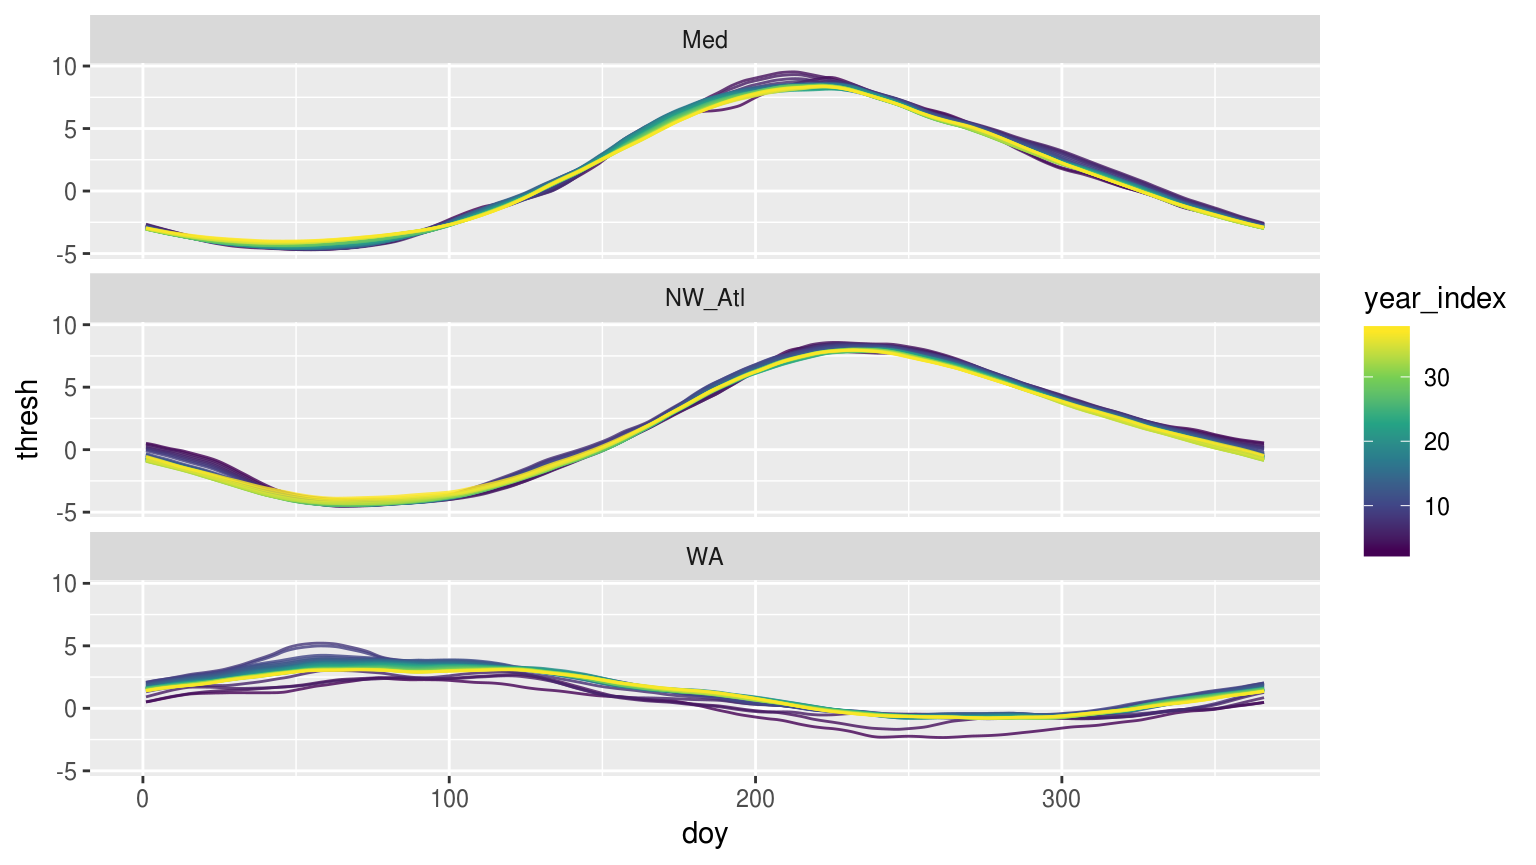
\includegraphics{../docs/articles/time_series_duration_files/figure-html/clim-ts-all-1.png}
\caption{Figure 1: Time series of each of climatology period used from
the original data shown overlapping one another to visualise how the
climatologies differ depending on the length of the climatology period
used.}
\end{figure}

\begin{figure}
\centering
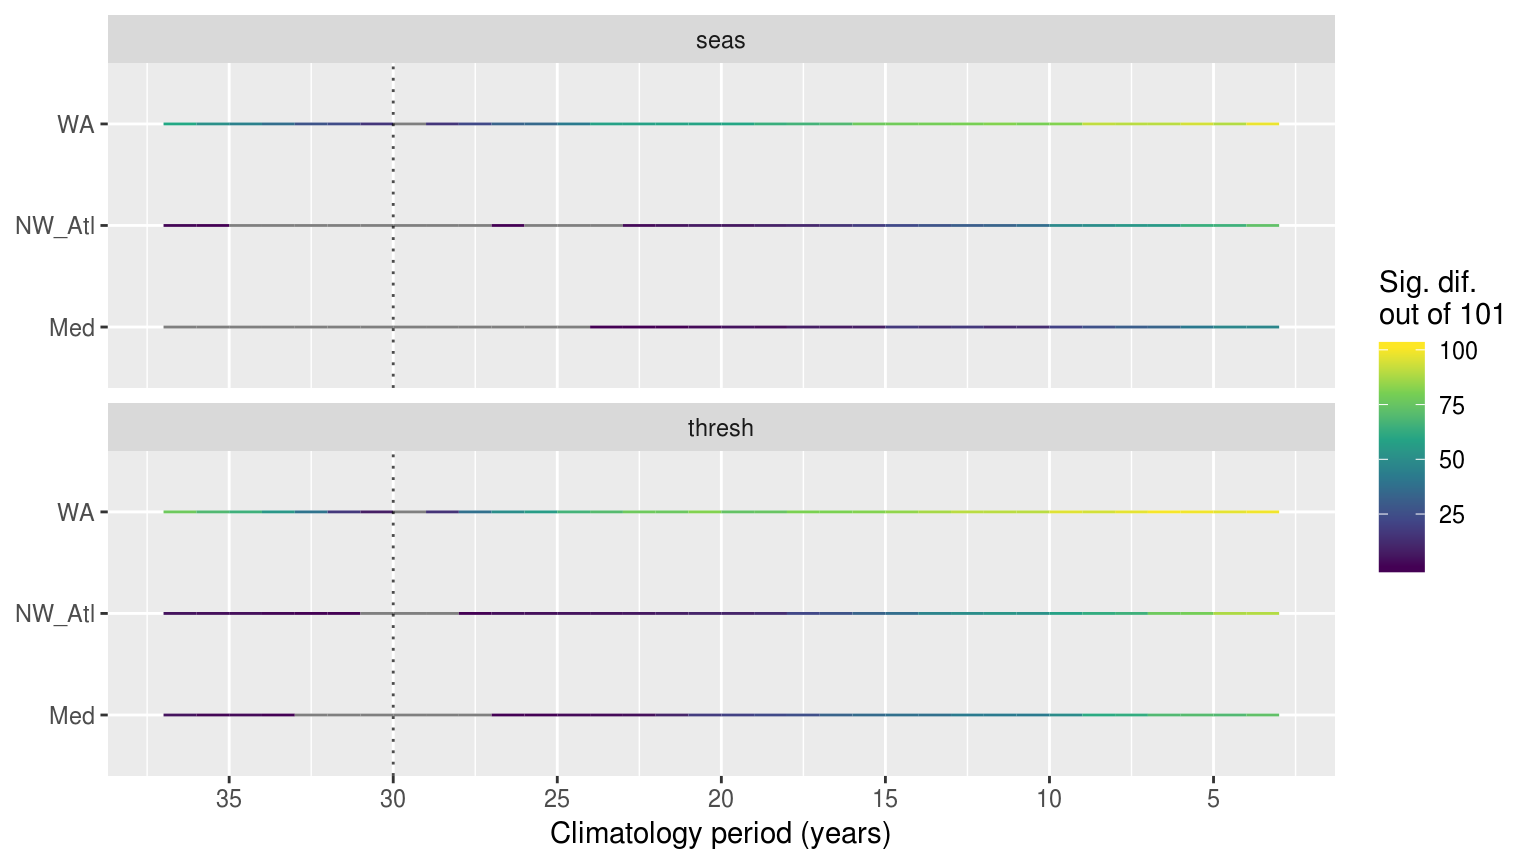
\includegraphics{../docs/articles/time_series_duration_files/figure-html/KS-clims-1.png}
\caption{Figure 2: Line plots showing the results of pairwise
Kolmogorov-Smirnoff tests for the seasonal signals (top panel) and 90th
percentile thresholds (bottom panel) from the same time series at
differing lengths. The colour of the line shows how many times out of
100 re-samples that the climatologies were significantly different from
the control. The dotted vertical line denotes the 30 year climatology
mark, against which all othe climatologies were compared. If no
re-samplings were significantly different this is shown with a grey
line.}
\end{figure}

\begin{itemize}
\tightlist
\item
  \emph{It may be better to show these results with a table as it would
  be easier to see when exactly the climatologies begin to differ.}
\end{itemize}

\paragraph{Alternative climatologies}\label{alternative-climatologies}

\begin{itemize}
\item
  \emph{I am thinking about removing this section due to time
  constraints.}
\item
  The investigation into the effect of
  \href{https://robwschlegel.github.io/MHWdetection/articles/Climatologies_and_baselines.html}{different
  methods} for calculating climatologies showed that, given certain
  circumstances, the accuracy of the threshold climatologies could be
  improved.
\end{itemize}

\begin{enumerate}
\def\labelenumi{\arabic{enumi}.}
\tightlist
\item
  The 7 basis function Fourier has very little variation over the entire
  year among the 100 simulations, but the dip during summer months is
  missed.
\item
  The 11 basis function Fourier gets some of the dip, but there is
  slightly more variation between the 100 simulations.
\item
  The MHW function's climatology captures the profile as it deviates
  away from a sinusoidal patterns better, but there is a large amount of
  variation between the randomisations.
\end{enumerate}

\subsubsection{Events}\label{events}

\begin{itemize}
\tightlist
\item
  The length of a time series had a negligible effect on the MHW metrics
  with only a few significant differences occurring at shorter time
  series
\item
  The post-hoc Tukey tests showed that no individual parings were
  significantly different
\item
  This is a surprising result

  \begin{itemize}
  \tightlist
  \item
    \emph{I double checked this but will triple check it}
  \end{itemize}
\end{itemize}

\subsubsection{Categories}\label{categories}

\begin{itemize}
\tightlist
\item
  The length of a time series had little effect on the count of
  categories

  \begin{itemize}
  \tightlist
  \item
    The largest count was for the \texttt{WA} at a time series length of
    10 being significantly different from 30 years only 5 times out of
    100.
  \end{itemize}
\end{itemize}

\begin{figure}
\centering
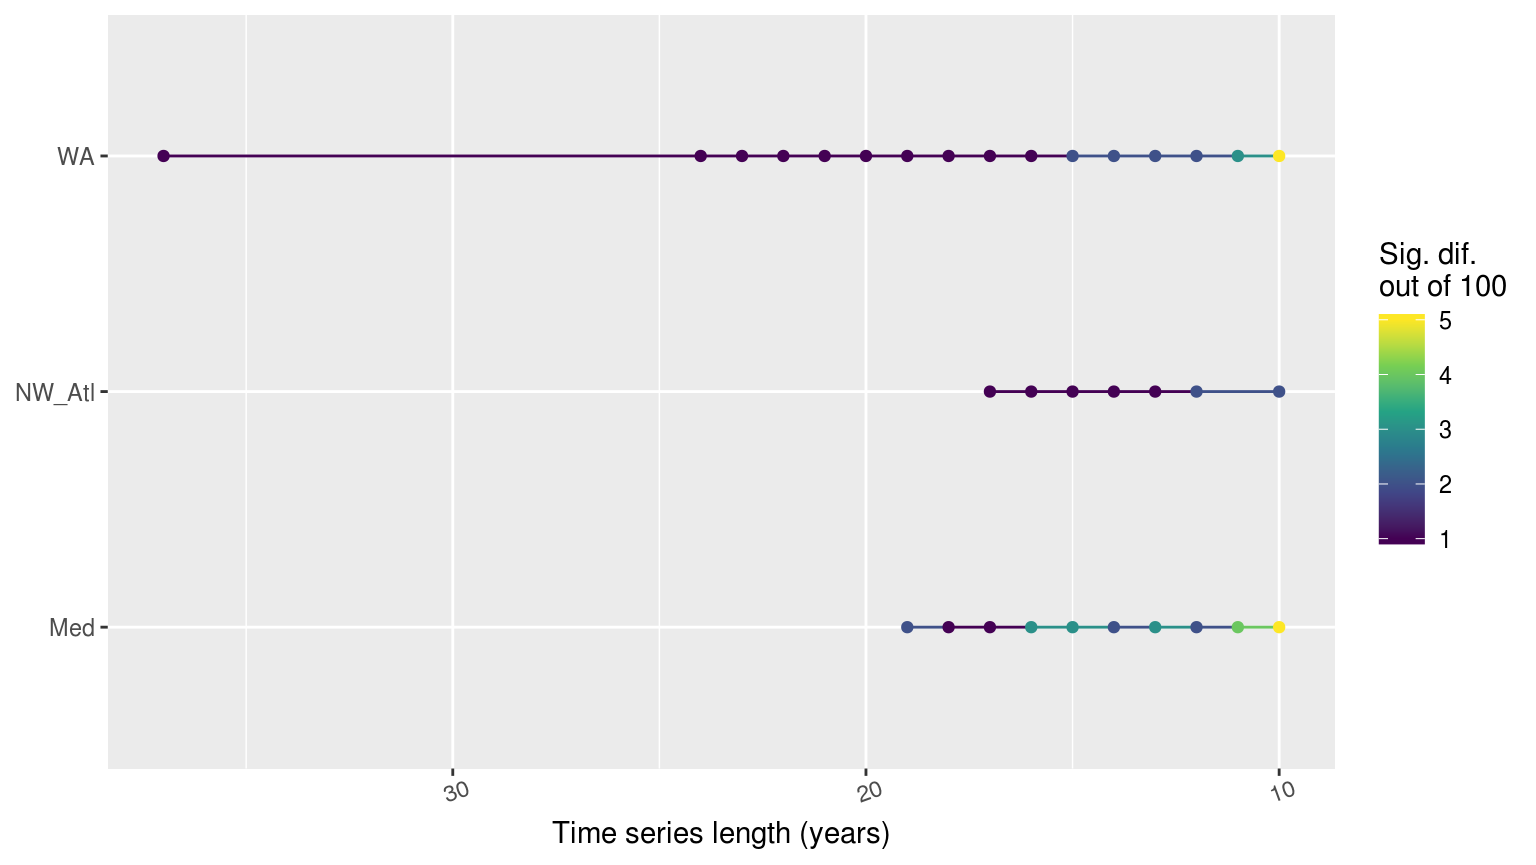
\includegraphics{../docs/articles/time_series_duration_files/figure-html/chi-pair-plot-1.png}
\caption{Figure 3: Line graph showing the count of times out of 100
random replicates when a given time series length led to significant
differences in the count of categories of MHWs as determined by a
\emph{chi}-squared test.}
\end{figure}

\subsection{Missing data}\label{missing-data}

\begin{itemize}
\tightlist
\item
  \emph{The detailed results are
  \href{https://robwschlegel.github.io/MHWdetection/articles/missing_data.html}{here}}
\end{itemize}

\subsubsection{Consecutive missing days}\label{consecutive-missing-days}

\begin{itemize}
\tightlist
\item
  The count of consecutive missing days increased with greater
  percentages of random missing data

  \begin{itemize}
  \tightlist
  \item
    The proportion of smaller consecutive missing days was logarithmic
    to the larger consecutive missing days
  \end{itemize}
\end{itemize}

\begin{figure}
\centering
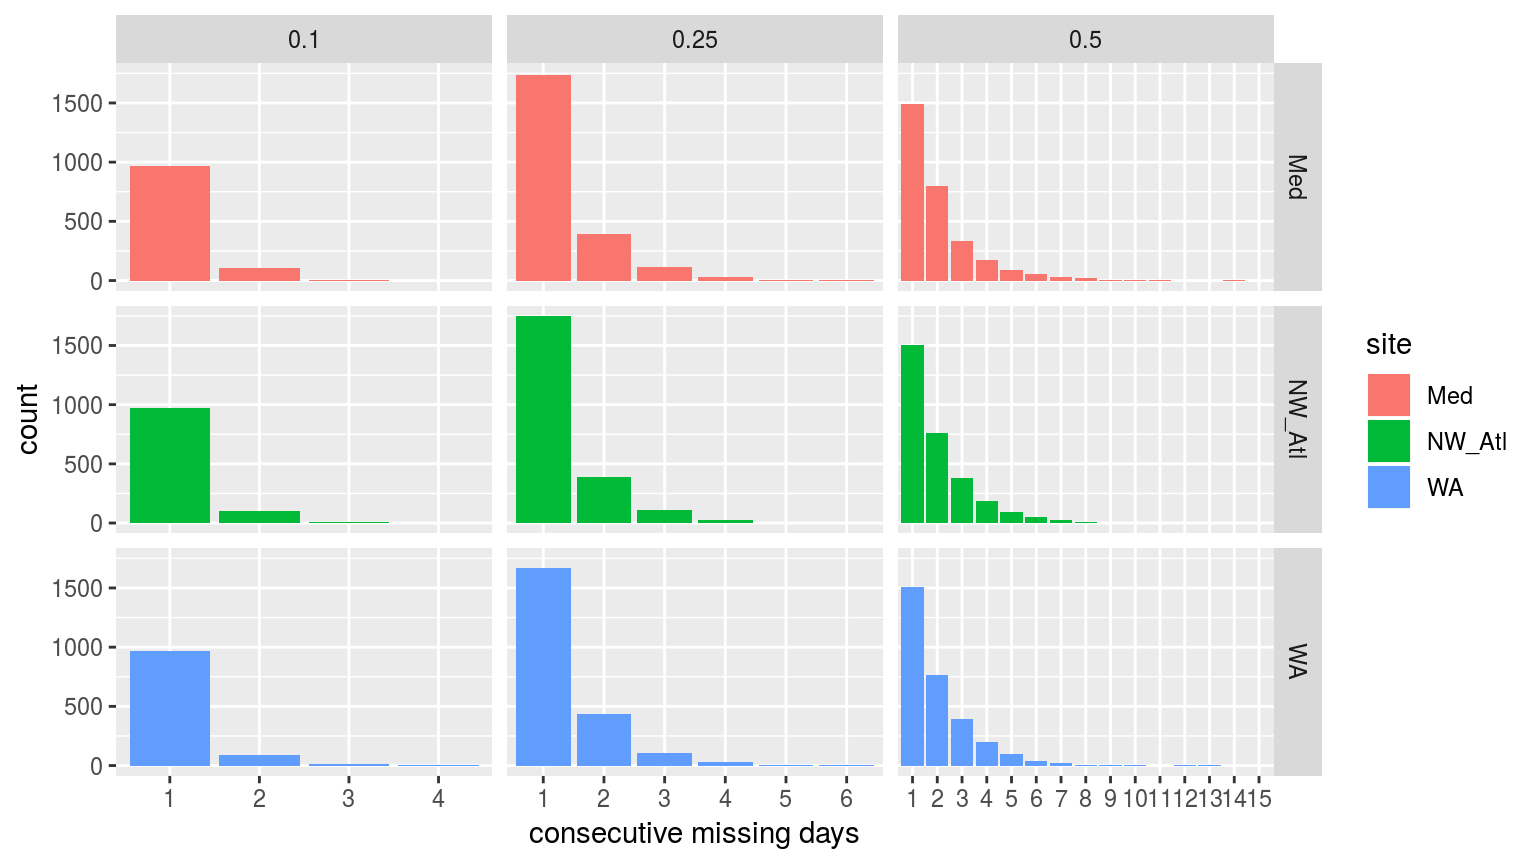
\includegraphics{../docs/articles/missing_data_files/figure-html/con-miss-1.png}
\caption{Figure 4: Dot and line plot showing the average count of
consecutive missing days of data as the percentage of missing data
increases. The colour scale is log transformed.}
\end{figure}

\subsubsection{Climatologies}\label{climatologies-1}

\begin{itemize}
\tightlist
\item
  Missing data had little perceptible effect on seasonal signals and
  produced only a few random significant differences with no clear
  pattern
\end{itemize}

\begin{figure}
\centering
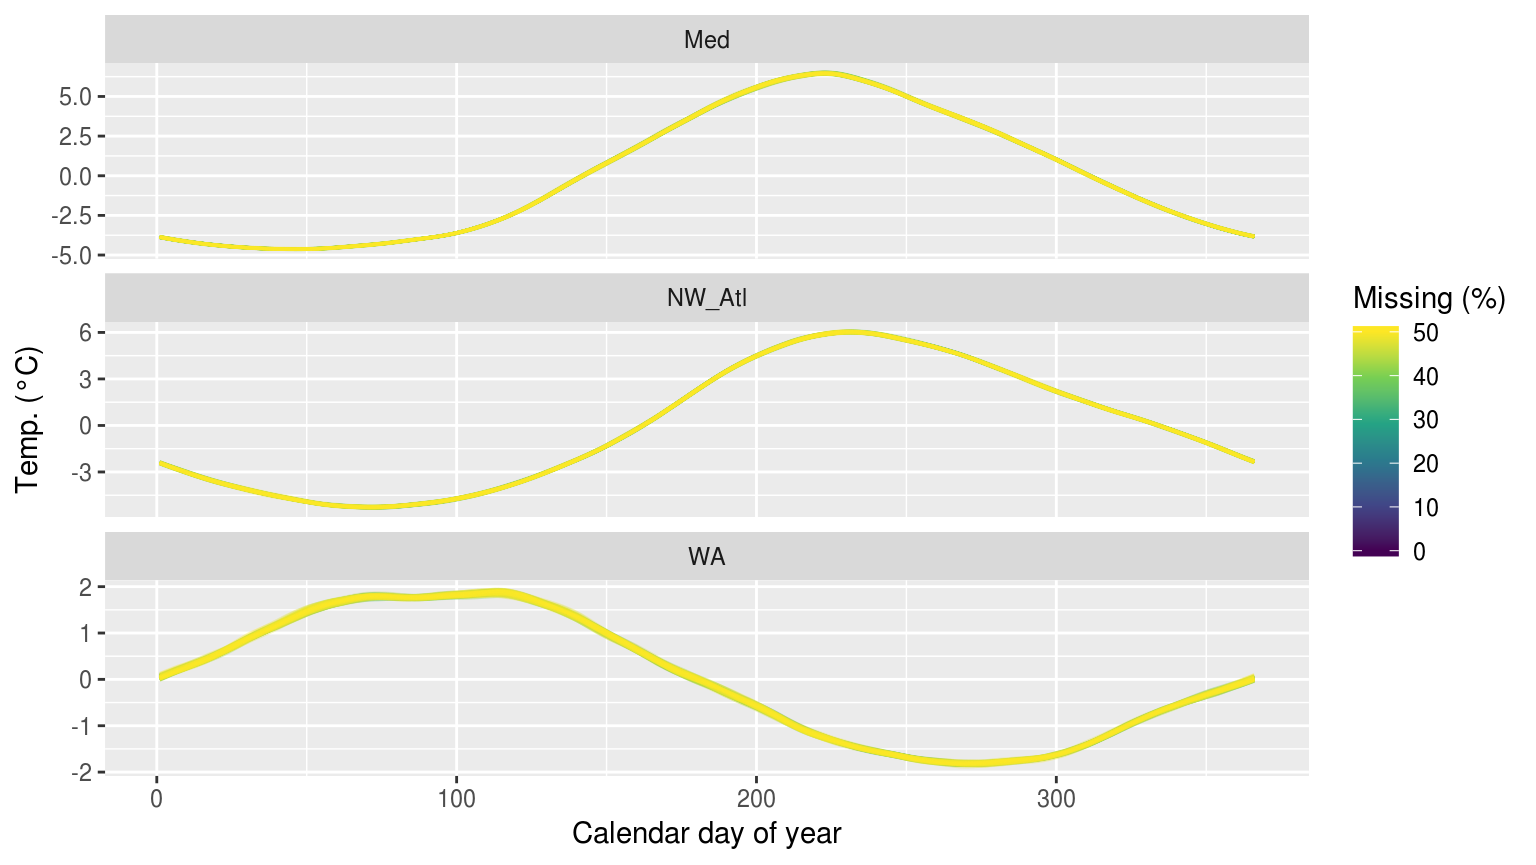
\includegraphics{../docs/articles/missing_data_files/figure-html/clim-miss-seas-1.png}
\caption{Figure 5: The seasonal signals created from time series with
increasing percentages of missing data.}
\end{figure}

\begin{itemize}
\tightlist
\item
  The effect of missing data on the threshold was obvious and usually
  significant
\end{itemize}

\begin{figure}
\centering
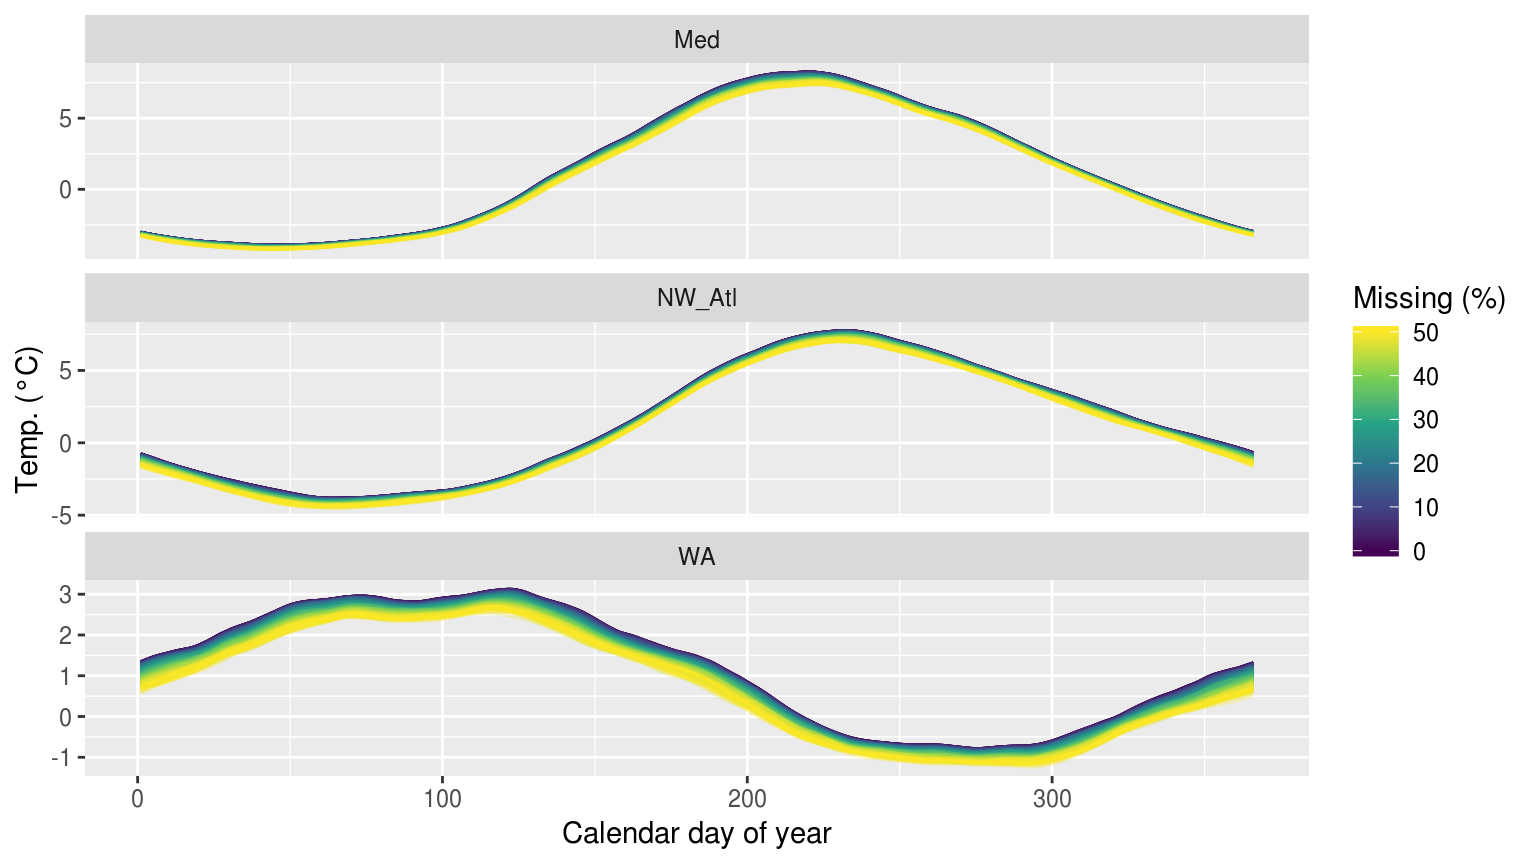
\includegraphics{../docs/articles/missing_data_files/figure-html/clim-miss-thresh-1.png}
\caption{Figure 6: The thresholds created from time series with
increasing percentages of missing data.}
\end{figure}

\begin{itemize}
\tightlist
\item
  Significant differences in thresholds from missing data differed
\item
  \texttt{WA} different at only 10\% missing data
\item
  \texttt{NW\_Atl} different at \textasciitilde{}23\%
\item
  \texttt{Med} not different until \textasciitilde{}29\%
\end{itemize}

\begin{figure}
\centering
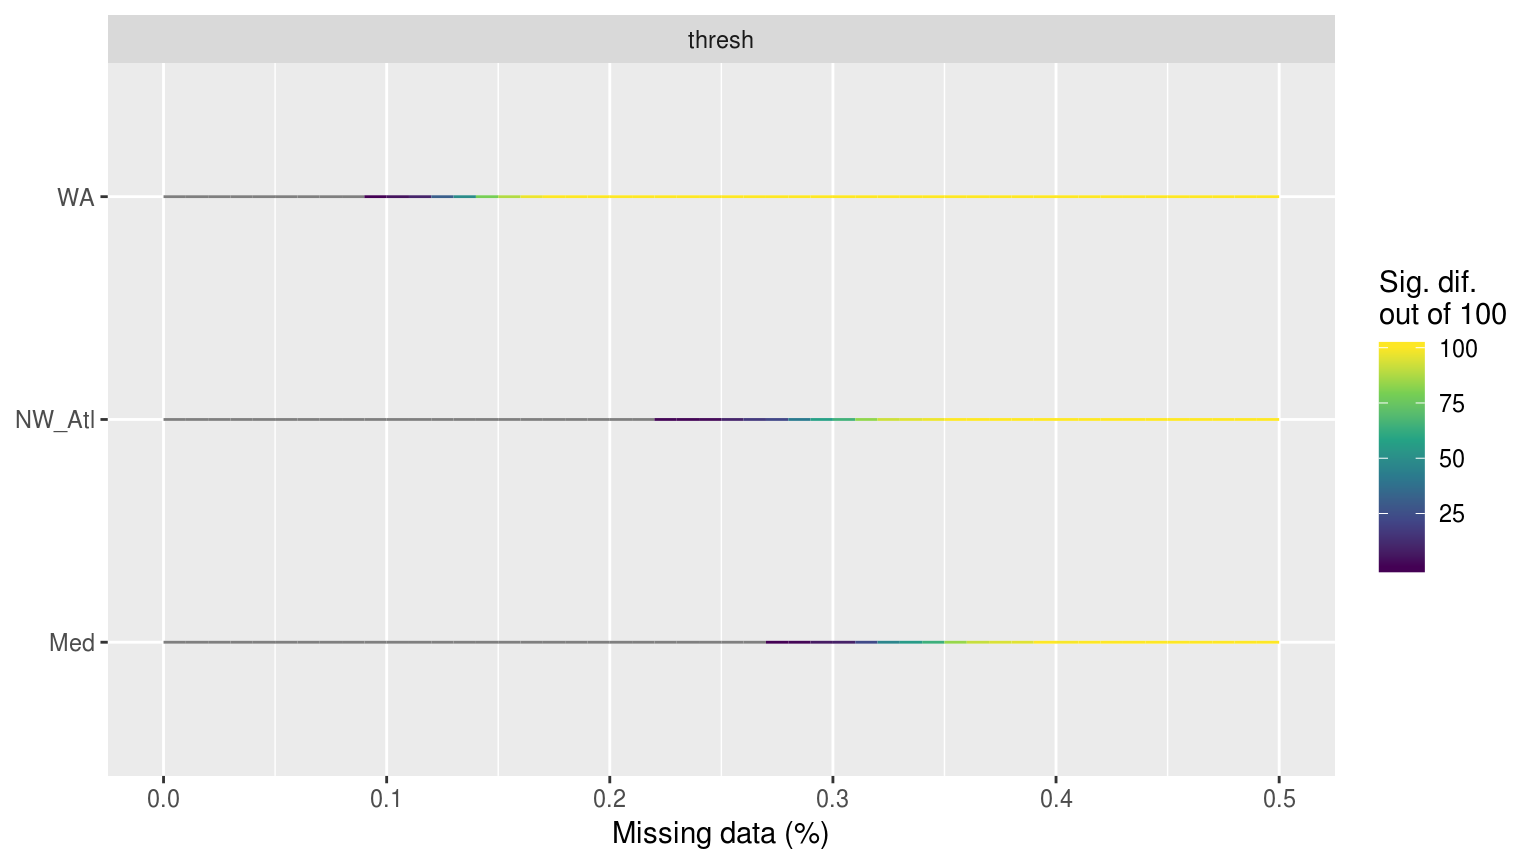
\includegraphics{../docs/articles/missing_data_files/figure-html/KS-clims-1.png}
\caption{Figure 7: Line plot showing the \emph{p}-value results from KS
tests comparing the distributions of each of the 100 replicated 90th
percentile thrsholds against the true (no missing data) climatologies
for each of the three reference time series.}
\end{figure}

\begin{itemize}
\tightlist
\item
  The count of 1 -- 3 consecutive missing days is a possible predictor
  of the threshold being significantly different from control
\end{itemize}

\begin{figure}
\centering
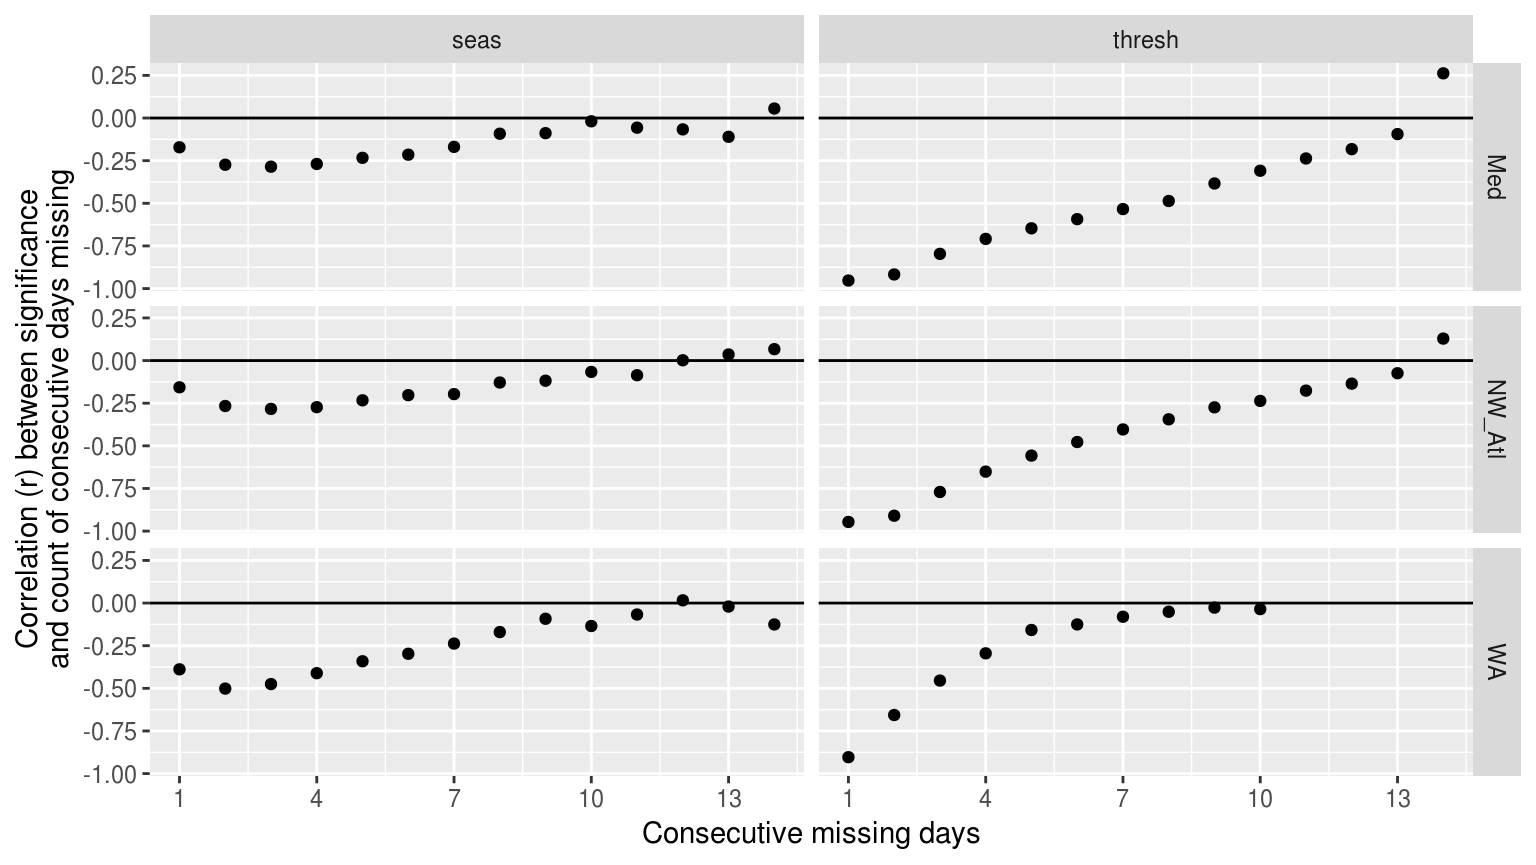
\includegraphics{../docs/articles/missing_data_files/figure-html/clim-cor-1.png}
\caption{Figure 8: Dot plot showing the relationship between number of
consecutive missing days and the significant difference of that
climatology as determined by KS tests. Consecutive missing days are a
much better predictor for thresholds than for seasonal signals.}
\end{figure}

\subsubsection{Events}\label{events-1}

\begin{itemize}
\tightlist
\item
  The time series proved to be remarkably resilient to missing data
  affecting the max and mean intensity of events

  \begin{itemize}
  \tightlist
  \item
    There was little effect, with missing percentages as large as 40\%
    being the most sensitivity observed
  \end{itemize}
\item
  The \texttt{WA} was the most resilient
\item
  The \texttt{NW\_Atl} was the most sensitive
\item
  Duration (and therefore cumulative intensity) became significantly
  different with as little as 10 -- 20\% missing data
\end{itemize}

\begin{figure}
\centering
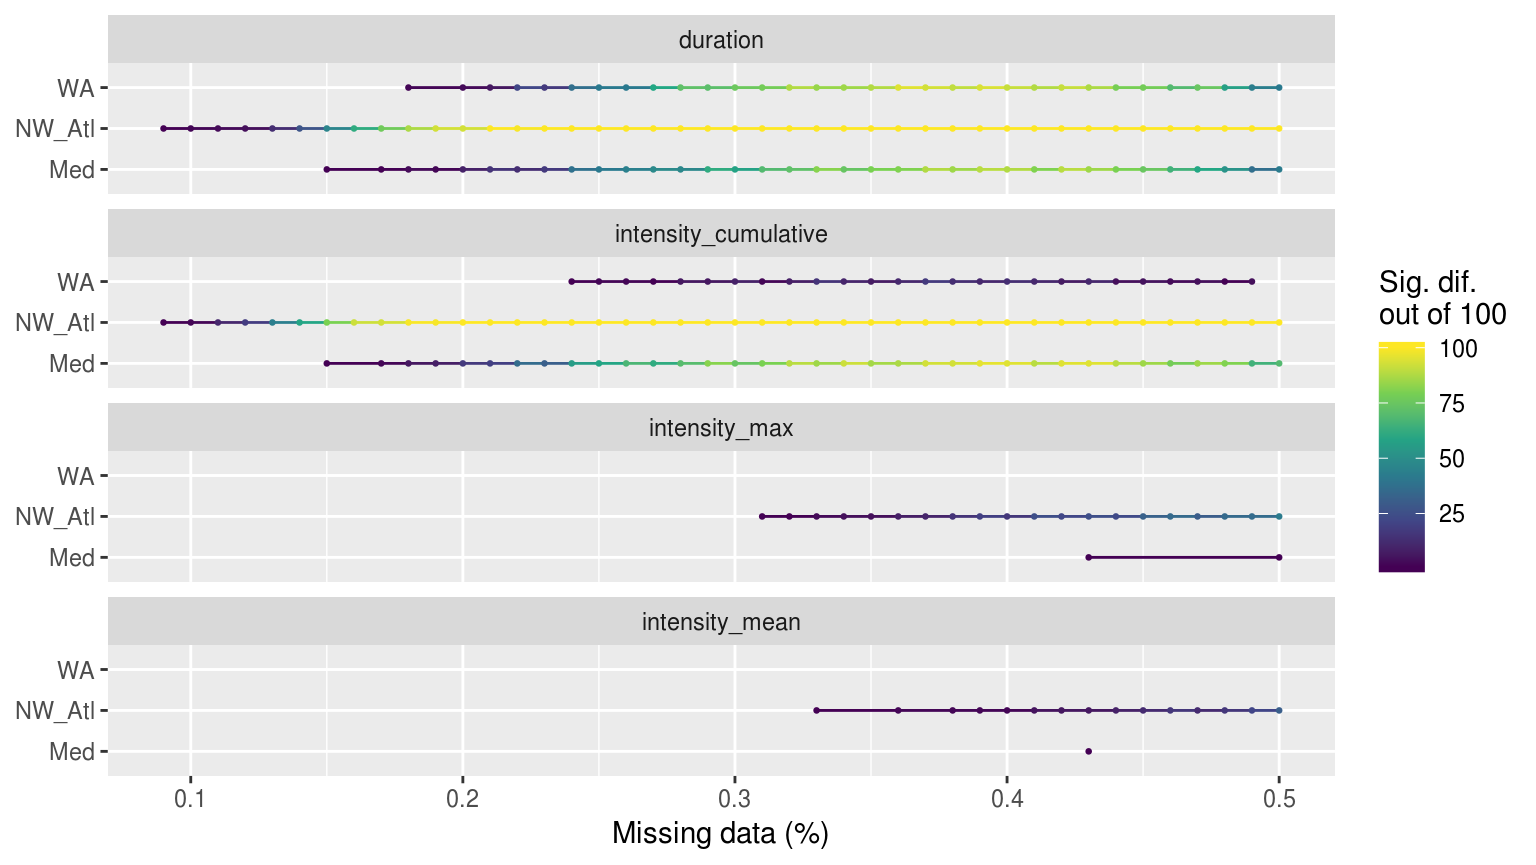
\includegraphics{../docs/articles/missing_data_files/figure-html/event-tukey-line-1.png}
\caption{Figure 9: Segments showing the range of the percent of missing
data present when climatologies were significantly different.}
\end{figure}

\begin{itemize}
\tightlist
\item
  Consecutive missing days appear to be a decent predictor for duration
  (and int. cum.) but not mean/max intensity
\end{itemize}

\begin{figure}
\centering
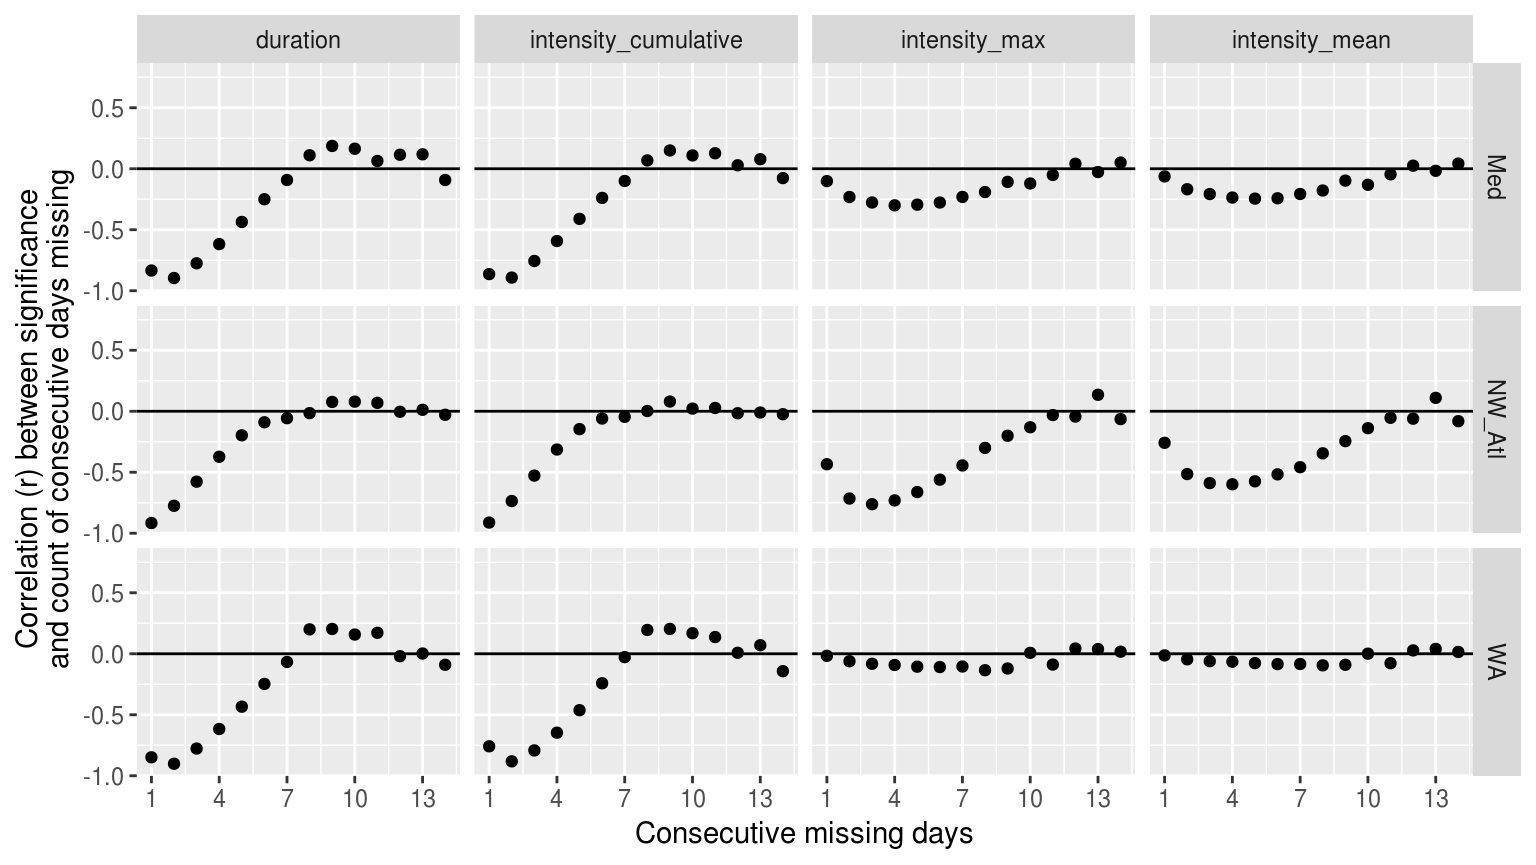
\includegraphics{../docs/articles/missing_data_files/figure-html/event-cor-1.png}
\caption{Figure 10: Dot plot showing the relationship between number of
consecutive missing days and the significant difference of the MHW
metric from the control.}
\end{figure}

\subsubsection{Categories}\label{categories-1}

\begin{itemize}
\tightlist
\item
  The \texttt{WA} was the most sensitive to missing data affecting
  category count, with the \texttt{Med} least sensitive
\item
  The range of missing data leading to significant differences in
  category count was \textasciitilde{}15 -- 25\%
\end{itemize}

\begin{figure}
\centering
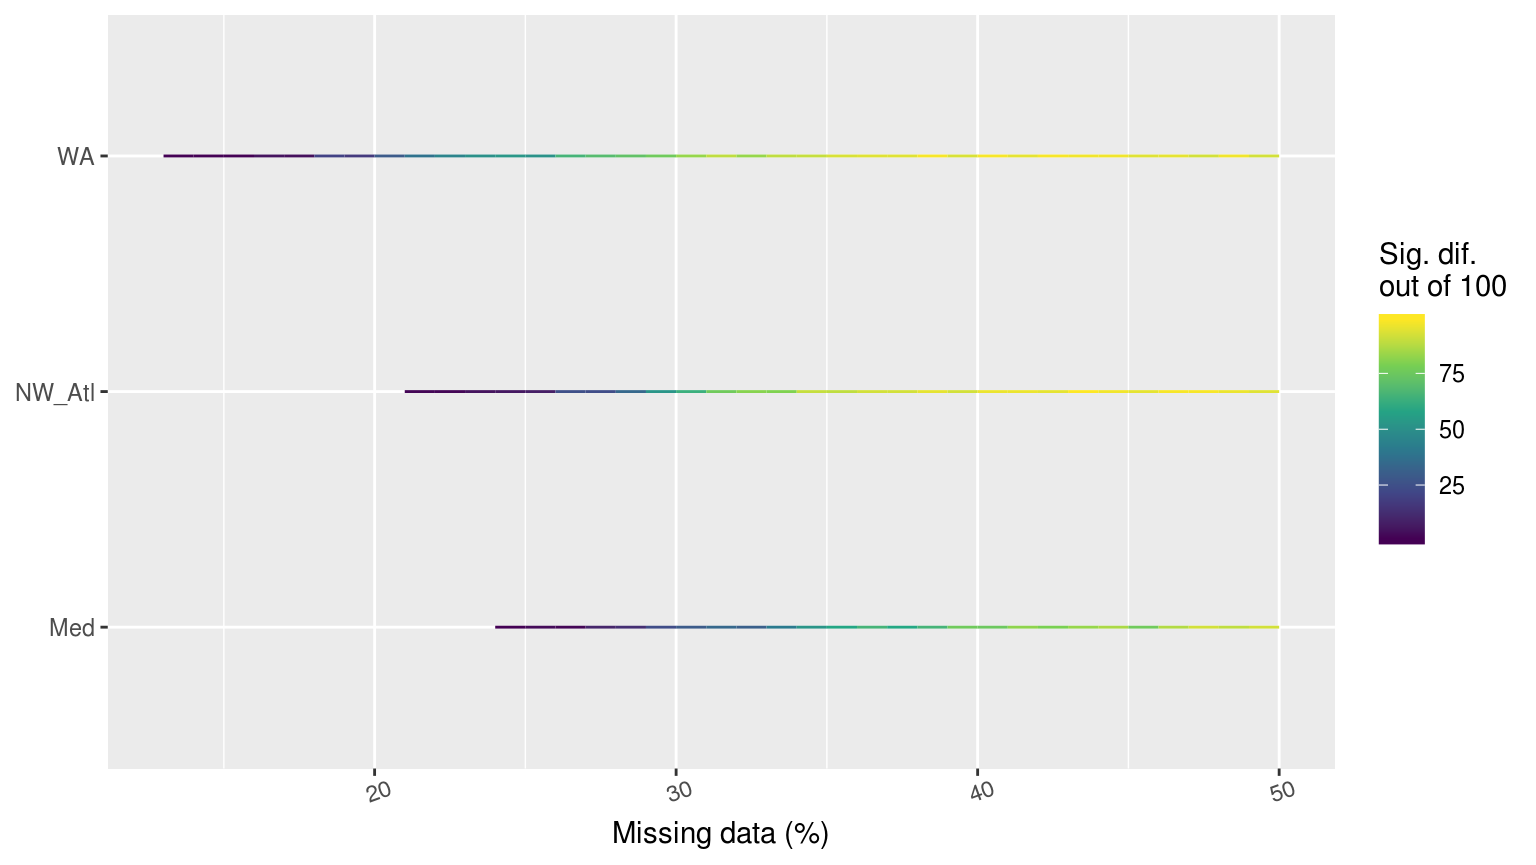
\includegraphics{../docs/articles/missing_data_files/figure-html/chi-pair-plot-1.png}
\caption{Figure 11: Line graph showing the count of times out of 100
random replicates when a given percentage of missing data led to
significant differences in the count of categories of MHWs as determined
by a \emph{chi}-squared test.}
\end{figure}

\begin{itemize}
\tightlist
\item
  \emph{Currently not showing the results of non-random missing data
  here.}

  \begin{itemize}
  \tightlist
  \item
    \emph{My thinking is to bring it up in the best practices section
    when the use of linear interpolation to deal with missing data is
    show cased.}
  \end{itemize}
\end{itemize}

\subsection{Long-term trends}\label{long-term-trends}

\begin{itemize}
\tightlist
\item
  \emph{The detailed results are
  \href{https://robwschlegel.github.io/MHWdetection/articles/trend.html}{here}}
\end{itemize}

\subsubsection{Climatologies}\label{climatologies-2}

\begin{itemize}
\tightlist
\item
  Adding decadal trends had a large effect on the \texttt{WA} seasonal
  signal
\end{itemize}

\begin{figure}
\centering
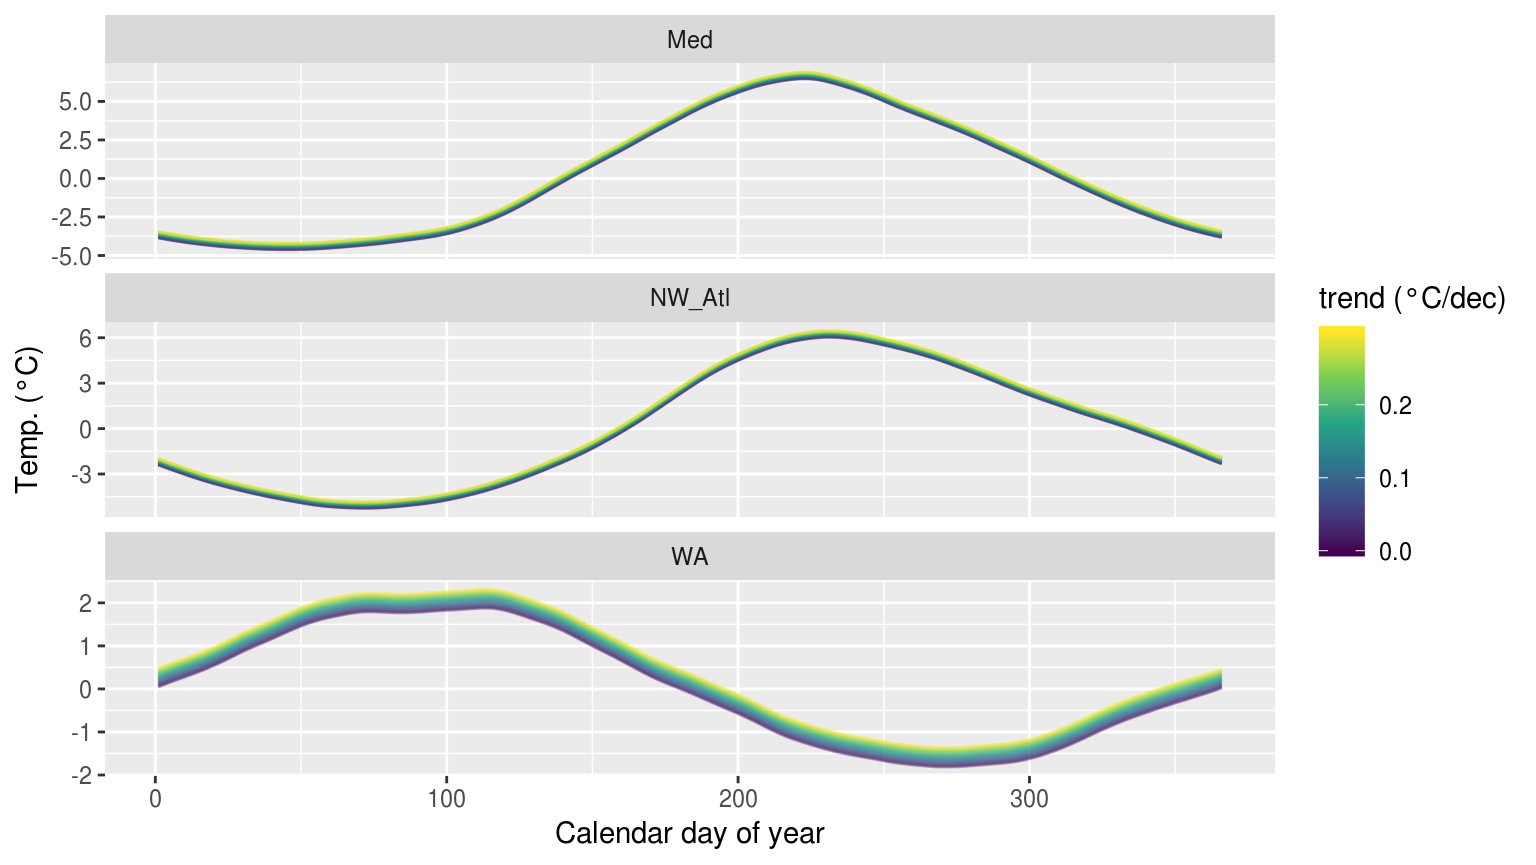
\includegraphics{../docs/articles/trend_files/figure-html/clim-trend-seas-1.png}
\caption{Figure 12: The seasonal signals created from time series with
increasingly large decadal trends added.}
\end{figure}

\begin{itemize}
\tightlist
\item
  Adding decadal trends had a smaller effect on the thresholds, which is
  interesting
\end{itemize}

\begin{figure}
\centering
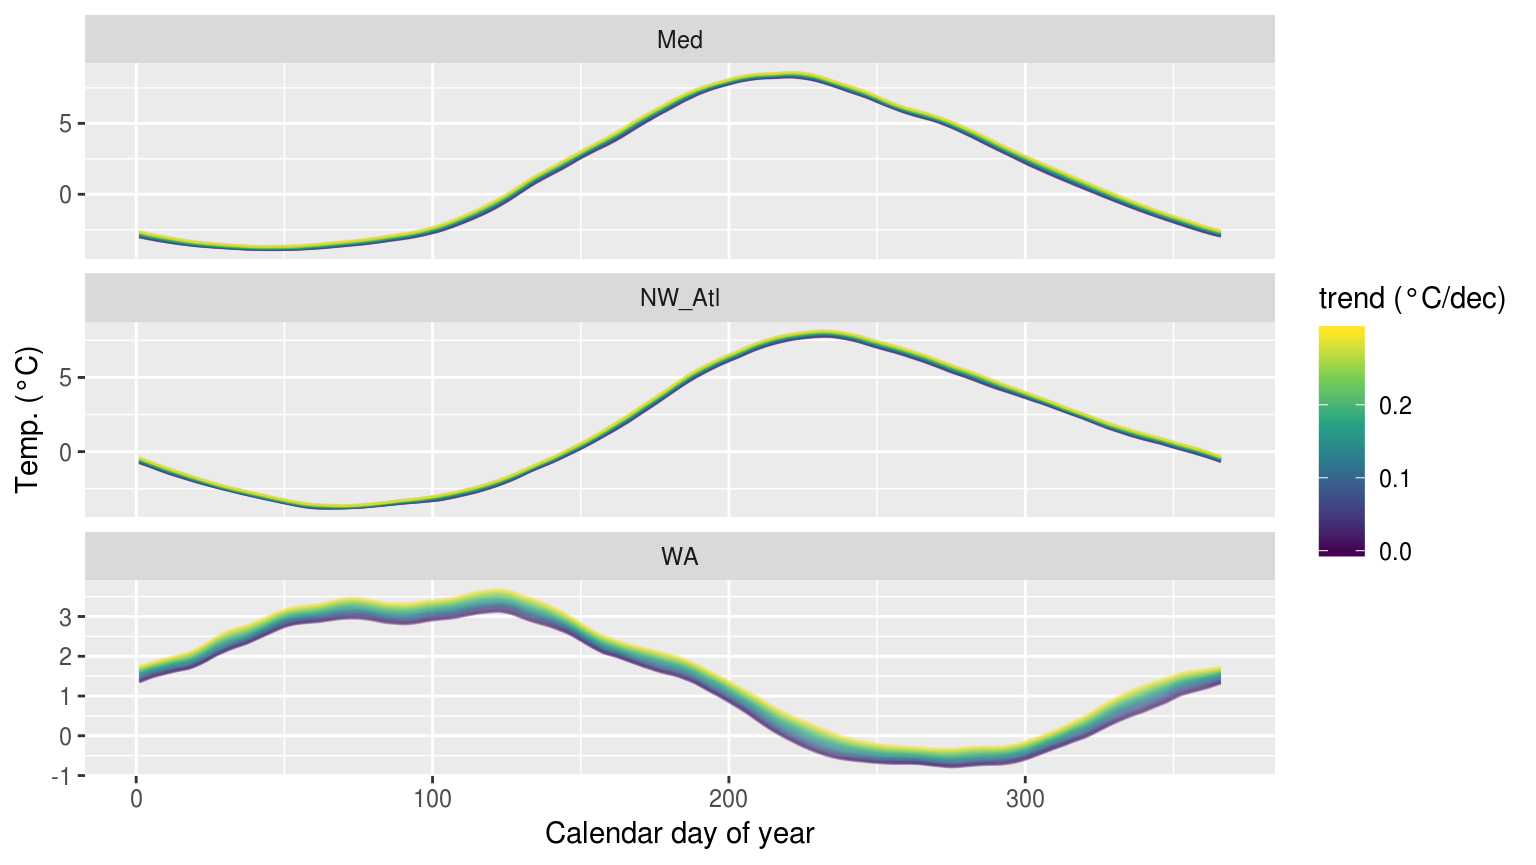
\includegraphics{../docs/articles/trend_files/figure-html/clim-trend-thresh-1.png}
\caption{Figure 13: The thresholds created from time series with
increasingly large decadal trends added.}
\end{figure}

\begin{itemize}
\tightlist
\item
  Depending on the time series, no amount of added decadal trend may
  make a difference
\end{itemize}

\begin{figure}
\centering
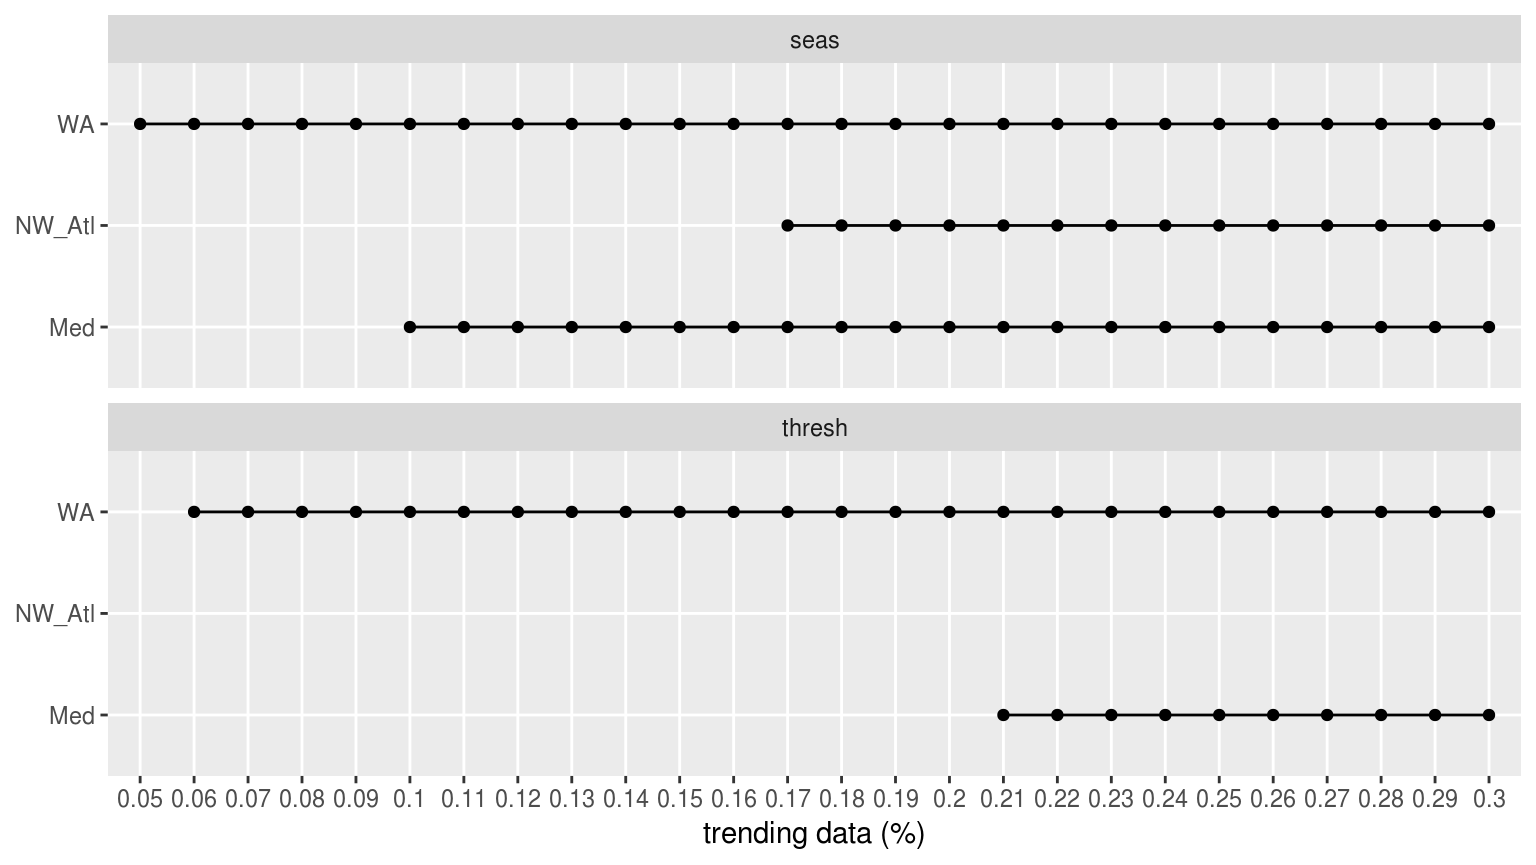
\includegraphics{../docs/articles/trend_files/figure-html/KS-clims-1.png}
\caption{Figure 14: Dot and line plot showing the \emph{p}-value results
from KS tests comparing the climatology statistics for increasingly
large decadal trends against the de-trended climatologies for each of
the three reference time series.}
\end{figure}

\subsubsection{Events}\label{events-2}

\begin{itemize}
\tightlist
\item
  No significant differences were detected
\end{itemize}

\subsubsection{Categories}\label{categories-2}

\begin{itemize}
\tightlist
\item
  The counts of categories did not differ significantly either
\end{itemize}

\section{Discussion}\label{discussion}

The fact that there is such a broad range across the results shows that
one must always exercise caution when using a sub-optimal time series.
But that with a healthy dose of caution there is still much that can be
done to ameliorate the issues outlined in the results.

\subsection{Time series length}\label{time-series-length}

\begin{itemize}
\tightlist
\item
  This is problematic
\end{itemize}

\subsection{Missing data}\label{missing-data-1}

\subsection{Long-term trends}\label{long-term-trends-1}

\subsection{Decision tree}\label{decision-tree}

\subsection{Best practices}\label{best-practices}

\begin{itemize}
\tightlist
\item
  \emph{After the investigation into the aforementioned topics has been
  completed, a series of best practices for dealing with these issues
  may be discussed}
\item
  \emph{We can provide guidelines about which suitable shorter time
  series data can/should be used for MHW detection, and how to select
  the best climatology creation method}
\item
  \emph{Ideally these could also be retroactively worked into the
  R/Python code to provide them as options for users}
\item
  \emph{Below is to be given an itemised list that readers could easily
  consult}
\end{itemize}

\subsubsection{De-trending}\label{de-trending}

\begin{itemize}
\tightlist
\item
  \emph{How/should a researcher account for a decadal trend when it is
  not technically possible to calculate one from a short time series?}

  \begin{itemize}
  \tightlist
  \item
    \emph{It could be advised that determining the trend from a nearby
    longer time series that shows good agreement could be done.}
  \end{itemize}
\end{itemize}

\subsubsection{Linear interpolation}\label{linear-interpolation}

\begin{itemize}
\tightlist
\item
  \emph{This is probably going to prove to be a silver bullet for most
  of the missing data issues}
\end{itemize}

\subsubsection{Climatology estimation
methods}\label{climatology-estimation-methods}

\begin{itemize}
\tightlist
\item
  \emph{For shorter time series, it might be better to use a more
  sinusoidal approximation of the climatology that captures the trend
  for the bulk of the year, but loses something around the deviations
  away from the perfect sine form}
\item
  \emph{Alternatively, if those deviations are seen as important
  features that need to be accounted for, then using the MHW climatology
  is probably better, but at the expense of overall accuracy}
\item
  \emph{We can provide an expert interpretation of the pros and cons of
  each method, and the technical tools to perform each method (through
  the code itself)}
\item
  \emph{That then leaves the user with expert recommendations and can
  make their own informed choice, given what they know about their data
  and what they want to prioritise/consider in their own analysis}
\item
  \emph{Also assess the effect of systematic varying windowHalfWidth and
  smoothPercentile and studying the outcomes for the three time series
  lengths}
\item
  \emph{Fourier transform climatologies/harmonic regression}
\item
  \emph{Analysis of short-duration, high resolution gridded SSTs}
\item
  \emph{It might be useful to show that in regions where events (at a
  certain threshold) can be detected in the dOISST data, that they also
  are present in the higher-res, shorter duration SST products}
\item
  \emph{Then we can show that in some scenarios the hi-res, short time
  series additionally capture some events that are not present in the
  OISST data due to its coarse spatial grid size}

  \begin{itemize}
  \tightlist
  \item
    \emph{compare reference time series vs.~other co-located SST data}
  \item
    \emph{compare in special conditions where events may be expected,
    but are not present in the dOISST data due to constraints resulting
    from it not being of high enough resolution; e.g.~in upwelling
    regions, embayments, etc}
  \end{itemize}
\end{itemize}

\subsubsection{Non-daily data}\label{non-daily-data}

\begin{itemize}
\tightlist
\item
  Some datasets come in weekly or monthly temporal resolution

  \begin{itemize}
  \tightlist
  \item
    These may be useful when daily data have too many NAs (e.g.~AVHRR
    Pathfinder, MODIS, and MERIS data)
  \item
    Can we use weekly and monthly data?
  \item
    What has been done along these lines?
  \item
    The way the R code is currently set-up, it will try to correct
    non-daily data into a daily time series with many gaps
  \item
    The problem then is that a time series will generally have about 1
    MHW per year by virtue of the 90th percentile threshold being used
  \item
    So if one uses monthly data it may be rather alarming to see that an
    area is experiencing month long MHWs every year
  \item
    The quick answer that comes to mind is to then play around with the
    `pctile' argument and see at what percentile threshold do different
    levels of super-daily data begin to match up with the 90th
    percentile on daily data
  \item
    Meaning, when there really is a month long MHW detected in daily
    data at a 90th percentile threshold, what must a comparable
    threshold be so that monthly data only `shows' a MHW at comparable
    times
  \end{itemize}
\end{itemize}

\subsection{Pitfalls}\label{pitfalls}

\begin{itemize}
\tightlist
\item
  \emph{What has been found that should be taken into consideration when
  using the above best practices}
\end{itemize}

\section{Conclusions}\label{conclusions}

\begin{itemize}
\item
  \emph{What are the main take away messages}
\item
  It looks like one can be pretty indelicate in choice of time series.
\item
  The MHW algorithm appears to be remarkably robust!
\end{itemize}

\section*{References}\label{references}
\addcontentsline{toc}{section}{References}

\hypertarget{refs}{}
\hypertarget{ref-Frolicher2018}{}
Frölicher, Thomas L, Erich M Fischer, and Nicolas Gruber. 2018. ``Marine
Heatwaves Under Global Warming.'' \emph{Nature} 560 (7718). Nature
Publishing Group: 360.

\hypertarget{ref-Garrabou2009}{}
Garrabou, J., R. Coma, N. Bensoussan, M. Bally, P. Chevaldonné, M.
Cigliano, D. Diaz, et al. 2009. ``Mass mortality in Northwestern
Mediterranean rocky benthic communities: effects of the 2003 heat
wave.'' \emph{Global Change Biology} 15 (5): 1090--1103.
doi:\href{https://doi.org/10.1111/j.1365-2486.2008.01823.x}{10.1111/j.1365-2486.2008.01823.x}.

\hypertarget{ref-Hobday2018}{}
Hobday, Alistair J, Eric CJ Oliver, Alex Sen Gupta, Jessica A
Benthuysen, Michael T Burrows, Markus G Donat, Neil J Holbrook, et al.
2018. ``Categorizing and Naming Marine Heatwaves.'' \emph{Oceanography}
31 (2). JSTOR: 162--73.

\hypertarget{ref-Hobday2016}{}
Hobday, Alistair J., Lisa V. Alexander, Sarah E. Perkins, Dan A. Smale,
Sandra C. Straub, Eric C.J. Oliver, Jessica A. Benthuysen, et al. 2016.
``A hierarchical approach to defining marine heatwaves.'' \emph{Progress
in Oceanography} 141: 227--38.
doi:\href{https://doi.org/10.1016/j.pocean.2015.12.014}{10.1016/j.pocean.2015.12.014}.

\hypertarget{ref-Oliver2018}{}
Oliver, Eric CJ, Markus G Donat, Michael T Burrows, Pippa J Moore, Dan A
Smale, Lisa V Alexander, Jessica A Benthuysen, et al. 2018. ``Longer and
More Frequent Marine Heatwaves over the Past Century.'' \emph{Nature
Communications} 9 (1). Nature Publishing Group: 1324.

\hypertarget{ref-Reynolds2007}{}
Reynolds, Richard W, Thomas M Smith, Chunying Liu, Dudley B Chelton,
Kenneth S Casey, and Michael G Schlax. 2007. ``Daily
high-resolution-blended analyses for sea surface temperature.''
\emph{Journal of Climate} 20 (22). NOAA, Natl Climatic Data Ctr,
Asheville, NC 28801 USA: 5473--96.


\end{document}
